\chapter{Preliminaries}
\section{Related Work}
\subsection{Video Inpainting} 
Recent advances in video inpainting have largely been driven by methods which fill in masked regions by borrowing content from the unmasked regions of other frames. These methods typically use optical flow estimates \citep{temporally, deepvideoinpainting, dfvi, flowedgeguided}, self-attention \citep{learningjoint, fuseformer, onionpeel, copypaste} or a combination of both \citep{propainter, fgt, endtoend} to determine how to propagate pixel values or learned features across frames. Such methods often produce visually compelling results, particularly on tasks where the mask-occluded region is visible in nearby frames such as foreground object removal. They struggle, however, in cases where this does not hold, for instance in the presence of heavy camera motion, large masks, or tasks where semantic understanding of the video content is required to produce a convincing result.

More recent work has utilized diffusion models for video inpainting. \citet{lookmanohands} uses a latent diffusion model \citep{stablediffusion, vahdat2021score} to remove the agent's view of itself from egocentric videos for applications in robotics. Notably, this is framed as an image inpainting task, where the goal is to remove the agent (with a mask provided by a segmentation model) from a single video frame conditioned on $h$ previous frames. Consequently, the results lack temporal consistency when viewed as videos, and the model is evaluated using image inpainting metrics only. \citet{avid} proposes a method for the related task of text-conditional video inpainting, which produces impressive results but requires user intervention. Most similar to this work, \citet{fgdvi} proposes a method for video inpainting that combines a video diffusion model with optical flow guidance. 


\subsection{Image Inpainting with Diffusion Models}
This work takes inspiration from the recent success of diffusion models for image inpainting. These methods can be split into two groups: those that inpaint using an unconditional diffusion model by making heuristic adjustments to the sampling procedure \citep{repaint, copaint}, and those that explicitly train a conditional diffusion model which, if sufficiently expressive and trained to optimality, enables exact sampling from the conditional distribution \citep{palette,zhang2023adding}. We follow the latter approach in this work.


\section{Background}
\subsection{Diffusion Models}
A diffusion model \citep{ddpm, sohldickstein} is comprised of two stochastic processes:  a forward (diffusion) process and a reverse (generative) process. Given a data distribution $q(\bx_0)$, the forward process, defined as
\begin{equation}
q (\bx_{0: T})=q(\bx_0) \prod_{t=1}^T q (\bx_t | \bx_{t-1} ), \quad q (\bx_t | \bx_{t-1} )=\mathcal{N} (\bx_t ; \sqrt{\alpha_t} \bx_{t-1}, (1-\alpha_t) \mathbf{I} ),
\end{equation}
gradually transforms this distribution into a prior distribution $q(\bx_T)$ through additive noise. Typically the noise schedule $\{\alpha_t\}_{t=1}^T$ is chosen such that $q(\bx_T) \approx \mathcal{N}(\mathbf{0},\mathbf{I})$. The reverse process, defined as 
\begin{equation}
p_\theta (\bx_{0: T} )=p (\bx_T ) \prod_{t=1}^T p_\theta (\bx_{t-1} | \bx_t ), \quad p_\theta (\bx_{t-1} | \bx_t )=\mathcal{N} (\bx_{t-1} ; \boldsymbol{\mu}_\theta (\bx_t, t ), \boldsymbol{\Sigma}_\theta (\bx_t, t ) )
\end{equation}
where $p(\bx_T) \defeq \mathcal{N}(\mathbf{0},\mathbf{I})$, is trained to match the joint distribution of the forward process by optimizing a variational lower bound. Here we adopt the reverse process parameterizations
\begin{equation}
    \boldsymbol{\mu}_\theta (\bx_t, t ) \defeq \frac{1}{\sqrt{\alpha_t}}\left(\mathbf{x}_t-\frac{1-\alpha_t}{\sqrt{1-\bar{\alpha}_t}} \boldsymbol{\epsilon}_\theta (\mathbf{x}_t, t)\right), \quad \boldsymbol{\Sigma}_\theta (\bx_t, t ) \defeq (1-\alpha_t)\mathbf{I}
\end{equation}
and simplified objective
\begin{equation}
    \mathcal{L}_{\text {simple }}(\theta):=\mathbb{E}_{t, \mathbf{x}_0, \boldsymbol{\epsilon}}\left[\left\|\boldsymbol{\epsilon}-\boldsymbol{\epsilon}_\theta\left(\sqrt{\bar{\alpha}_t} \mathbf{x}_0+\sqrt{1-\bar{\alpha}_t} \boldsymbol{\epsilon}, t\right)\right\|^2\right]
    \label{eq:lsimple-ddpm}
\end{equation}
 of \citet{ddpm}, where $\bar{\alpha}_t:=\prod_{s=1}^t \alpha_s$, $\mathbf{x}_0 \sim q(\bx_0)$, $t \sim \text{Unif}(\{1, \ldots, T\})$,  $\boldsymbol{\epsilon} \sim \mathcal{N}(\mathbf{0},\mathbf{I})$, and $\boldsymbol{\epsilon}_\theta$ is a neural network trained to predict the noise $\boldsymbol{\epsilon}$ added to $\bx$ conditioned on $t$.
\subsection{Conditional Diffusion Models}
This framework is easily extended to conditional generation tasks where we wish to model $p(\bx_0|\by)$ for some conditioning signal $\by$, for instance the unmasked regions of an image in the case of image inpainting \citep{palette}. The reverse process is modified to condition on $\by$ in the transition densities $p_\theta(\bx_{t-1}|\bx_t, \by)$, typically by including $\by$ as an input to the neural network: $\boldsymbol{\epsilon}_\theta(\bx_t, \by, t)$. The data distribution becomes a joint distribution $q(\bx_0, \by)$, and \Cref{eq:lsimple-ddpm} is modified accordingly:		
\begin{equation}
    \mathcal{L}_{\text {cond }}(\theta):=\mathbb{E}_{t, \mathbf{x}_0, \mathbf{y}, \boldsymbol{\epsilon}}\left[\left\|\boldsymbol{\epsilon}-\boldsymbol{\epsilon}_\theta\left(\sqrt{\bar{\alpha}_t} \mathbf{x}_0+\sqrt{1-\bar{\alpha}_t} \boldsymbol{\epsilon}, \mathbf{y}, t\right)\right\|^2\right].
    \label{eq:lcond}
\end{equation}
Once such the network has been trained, various methods exist for using it to draw approximate samples from $p(\mathbf{x}_0|\mathbf{y})$ \citep{ddpm,sohldickstein,tashiro2021csdi,song2020score,karras2022elucidating}. We use the Heun sampler proposed by \citet{karras2022elucidating}, and leave further details to the appendix.

\begin{figure}[t]
    \centering
    \begin{subfigure}[t]{0.3\textwidth}
        \centering
        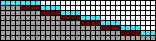
\includegraphics[width=\textwidth]{figures/sampling-scheme-visualizations/autoreg.png}
        \caption{AR}
        \label{fig:ar}
    \end{subfigure}
    ~
    \begin{subfigure}[t]{0.3\textwidth}
        \centering
        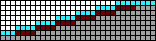
\includegraphics[width=\textwidth]{figures/sampling-scheme-visualizations/reverse-autoreg.png}
        \caption{Reverse AR}
        \label{fig:rev_ar}
    \end{subfigure}
    ~
    \begin{subfigure}[t]{0.3\textwidth}
        \centering
        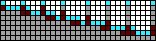
\includegraphics[width=\textwidth]{figures/sampling-scheme-visualizations/hierarchy-2.png}
        \caption{Hierarchy-2}
        \label{fig:h2}
    \end{subfigure}
    \caption[A visualization of sampling schemes introduced in prior work.]{A visualization of sampling schemes (introduced in \citet{fdm}) for generating videos of length $N=31$ while accessing only $K=8$ frames at a time. Each row of each subfigure depicts a different stage of our sampling process, starting from the top row and working down. Each column represents one video frame. Within each stage, frames shown in \textcolor{latentcolor}{cyan} are being sampled conditioned on the values of previously-sampled frames shown in \textcolor{observedpastcolor}{dark red}. Frames shown in white are not yet generated. By the end, all frames are generated and shown in \textcolor{completecolor}{light gray}.
    }
    \label{fig:old-sampling-schemes}
\end{figure}


\subsection{Video Diffusion Models}
Before we discuss conditional video diffusion models, we first discuss video diffusion models in general. A number of recent papers have proposed diffusion-based approaches to generative modeling of video data \citep{didrik, fdm, vdm, yang2022diffusion, voleti2022MCVD}. 
We follow the majority of these approaches \citep{fdm,vdm,voleti2022MCVD} in using a 4-D U-Net~\citep{unet} architecture to parameterize $\boldsymbol{\epsilon}_\theta(\ldots)$. 
Alternating spatial and temporal attention blocks within the U-Net capture dependencies within and across frames respectively, with relative positional encodings \citep{rpe1, rpe2} providing information about each frame's position within the video. 
Due to computational constraints, video diffusion models are inherently limited to conditioning on and generating a small number of frames at a time, which we denote as $K$. 

\subsection{Flexible Video Diffusion Models}
Generating long videos with numbers of frames $N \gg K$ then requires sampling from the diffusion model multiple times. A typical approach would be to break the generation down into multiple stages, and in each stage sample $K/2$ frames conditioned on the previous $K/2$ frames. 
We depict this approach in \Cref{fig:ar}, with each row representing one stage. A problem with this strategy is that it fails to capture dependencies on frames more than $K/2$ frames in the past. 
Alternative orders in which to generate frames (which we will refer to as ``sampling schemes'') are possible, with some additional ones depicted in \Cref{fig:h2,fig:rev_ar}. Each of these sampling schemes tends to have its downsides, and experimentation usually requires expensive retraining of models. 
\citet{fdm} therefore suggest training a single model that can perform well on any sampling scheme. In particular, they train a model to generate any subset of video frames conditioned on any other subset with the objective
\begin{equation}
    \mathcal{L}_{\text {flexible}}(\theta):=\mathbb{E}_{t, \mathbf{x}, \mathbf{y}, \mathcal{X}, \mathcal{Y}, \boldsymbol{\epsilon}}\left[\left\|\boldsymbol{\epsilon}-\boldsymbol{\epsilon}_\theta\left(\sqrt{\bar{\alpha}_t} \mathbf{x}+\sqrt{1-\bar{\alpha}_t} \boldsymbol{\epsilon}, \mathbf{y}, \mathcal{X}, \mathcal{Y}, t\right)\right\|^2\right],
    \label{eq:lflexible}
\end{equation}
in which $\mathbf{x}$ are the frames to remove noise from at indices $\mathcal{X}$, and $\mathbf{y}$ are the frames to condition on at indices $\mathcal{Y}$. 
To sample $\mathbf{x}$ and $\mathbf{y}$ we first sample $\mathcal{X}$ and $\mathcal{Y}$, then sample a training video, and then extract the frames at indices $\mathcal{X}$ and $\mathcal{Y}$ to form $\mathbf{x}$ and $\mathbf{y}$, respectively.
Both the number of frames to generate and the number to condition on can vary, so the shapes of $\mathbf{x}$, $\boldsymbol{\epsilon}$, and $\mathbf{y}$ can vary correspondingly. The network is given the indices of all frames ($\mathcal{X}$ and $\mathcal{Y}$), as they are used to create the relative positional encodings \citep{rpe1, rpe2}. 
Once a network is trained to make predictions for arbitrary indices $\mathcal{X}$ given arbitrary indices $\mathcal{Y}$, it can be used to sample long videos with any desired sampling scheme. Sampling schemes will henceforth be denoted as $\{\mathcal{X}_s, \mathcal{Y}_s\}_{s=1}^S$ where $S$ is the number of sampling stages and, at stage $s$, $\mathcal{X}_s$ and $\mathcal{Y}_s$ are the indices of the latent and observed frames, respectively. 











